\documentclass[12pt]{article}
\textwidth 15.5cm \oddsidemargin 0cm \topmargin -1cm \textheight 24cm \footskip 1.5cm
\usepackage{epsfig, amsmath,graphicx,psfrag,pstcol, float, listings, caption, array, verbatim}
\newenvironment{metaverbatim}{\verbatim}{\endverbatim}
\def\n{\noindent}
\def\u{\underline}
\def\hs{\hspace}
\newcommand{\thrfor}{.^{\displaystyle .} .}
\newcommand{\bvec}[1]{{\bf #1}}
\captionsetup{justification=centering, width=0.5\textwidth}
\title{GF2: Software First Interim Report}
\author{Team 7\\Z.Wang(zw296)\\S.Yuchi(sy334)\\Z.Gu(zg245)}

\begin{document}
\maketitle

\vspace{80mm}
\section{Introduction}
The report focuses on the planning of the whole project in terms of task assignments and time planning. The project is divided into a number of 
tasks including design and implementation, for which the time lines are set in order to allow time for integration and testing by another team number. Additionally the report 
addresses the design of syntax grammar in EBNF language, which will be adhered to throughout the project. It also describes the identification 
and handling for both syntax and semantic errors. Two examples of the definition files and corresponding setups are appended.

\newpage
\section{General Approach}
It is agreed that the pattern of the grammar syntax must be complied throughout the construction of the project. Since there are a few blocks of the programme which have already been given, it is expected to be modified adequately in order to fit the team's design on scanner and parser wherever necessary. The time allocation is expected to allow time for integration of the programme from each functions and the testing of individual functionality by the other team members.

\section{Teamwork planning}
\subsection{Interface design for scanner and GUI}
Designed by the whole team, before Tuesday 23 May.

\subsection{$Names$ class implementation}
Implementation already finished by Zhiwei.\\
Testing finished by Zhengyang before Tuesday 30 May.

\subsection{$Scanner$ class implementation}
Implementation finished by Shaowu before Saturday 27 May.\\
Testing finished by Zhiwei before Tuesday 30 May.

\subsection{$Parser$ class implementation}
Implementation finished by Zhiwei and Zhengyang before Saturday 27 May.\\
Testing finished by Shaowu before Tuesday 30 May.

\subsection{$GUI$ class implementation}
Implementation finished by Zhiwei and Shaowu before Saturday 27 May.\\
Testing finished by Zhengyang before Tuesday 30 May.

\subsection{System integration}
Integration and testing by the whole team, before the deadline of the second interim report (Friday 2 June).

\subsection{System maintenance}
Modification and testing by the whole team, before the deadline of the final report (Thursday 8 June).

\newpage
\section{Syntax in EBNF language}
\begin{metaverbatim}
file =  `DEVICES', DEV, {`,', DEV}, `;', `CONNECT', CON, {`,', CON}, `;',
        `MONITOR', MON, {`,', MON}, `;';
DEV  =  `CLOCK', DEV_NAME, digit, {digit} |
        `SWITCH', DEV_NAME, ( 1 | 0 ) |
        `AND' | `NAND' | `OR' | `NOR', DEV_NAME, [1], digit	|
        `D_TYPE', DEV_NAME |
        `XOR', DEV_NAME;
DEV_NAME  =	 (digit | letter | `_'), {digit | letter | `_'};
CON       =  O_PIN, `=>', I_PIN;
O_PIN     =  DEV_NAME |
             DEV_NAME, `.Q', [`BAR'];
I_PIN     =  DEV_NAME, `.I', [1], digit	|
             DEV_NAME, `.', (`DATA'|`CLK'|`SET'|`CLEAR');
MON       =  O_PIN | I_PIN;

letter = "A" | "B" | "C" | "D" | "E" | "F" | "G"
       | "H" | "I" | "J" | "K" | "L" | "M" | "N"
       | "O" | "P" | "Q" | "R" | "S" | "T" | "U"
       | "V" | "W" | "X" | "Y" | "Z" | "a" | "b"
       | "c" | "d" | "e" | "f" | "g" | "h" | "i"
       | "j" | "k" | "l" | "m" | "n" | "o" | "p"
       | "q" | "r" | "s" | "t" | "u" | "v" | "w"
       | "x" | "y" | "z" ;
digit = "0" | "1" | "2" | "3" | "4" | "5" | "6" | "7" | "8" | "9" ;

\end{metaverbatim}

\newpage
\section{Syntax error identification and handling}
\begin{center}
	\begin{tabular}{|m{3cm} | m{6cm} | m{8cm} |}
		\hline
		Error Name & Identification & Handling \\
		\hline
		Input Connected to Input & I\_PIN =\textgreater  I\_PIN under CONNECT &  Report, syntax error count + 1, continue parsing, cancel simulation \\
		\hline
		Input Connected to Output & I\_PIN =\textgreater  O\_PIN under CONNECT &  Report, syntax error count + 1, continue parsing, cancel simulation \\
		\hline
		Output Connected to Output & O\_PIN =\textgreater  O\_PIN under CONNECT &  Report, syntax error count + 1, continue parsing, cancel simulation \\
		\hline
		No Device Found & Empty DEVICE section & Report, syntax error count + 1, continue parsing, cancel simulation \\
		\hline
		No Connection Found & Empty CONNECT section & Report, syntax error count + 1, continue parsing, cancel simulation \\
		\hline
		No Monitor Found & Empty MONITOR section & Report, syntax error count + 1, continue parsing, cancel simulation \\
		\hline
		Undefined Object & Device used in CONNECT or MONITOR not found in the symbol table & Report, syntax error count + 1, continue parsing, cancel simulation \\
		\hline
		Unexpected Token & When the type of token does not match the expected type, e.g. 
		
		1. too many parameters after DEVICE definition; 
		
		2. second `=\textgreater' found in a CON statement; 
		
		3. missing `,' or `;';  
		
		essentially anything violates the syntax defined in the previous section
		& Report, Report Token type expected,  syntax error count + 1, continue parsing from next valid statement (jump to the next `,' or `;', whichever is closer), cancel simulation \\
		\hline
	
	\end{tabular}
\end{center}
\newpage
\section{Semantics error identification and handling}
\begin{center}
	\begin{tabular}{|m{3cm} | m{6cm} | m{8cm} |}
		\hline
		Error Name & Identification & Handling \\
		\hline
		Floating Input & Input of a device is not connected to any output. Check using $checknetwork$ after CONNECT section is parsed & Report, semantic error count +1, continue parsing,  cancel simulation \\
		\hline
		Unused Output & Output of a device is not connected to any input or monitored. Check after MONITOR section is parsed. & Report, semantic warning count +1, continue parsing \\
		\hline
		Multiple Output Connected to Single Input Pin & Check if an input pin is referred to twice under CONNECT section after CONNECT section is parsed & Report, semantic error count +1, continue parsing,  cancel simulation \\
		\hline
		Invalid Clock Period (T$\leq$0) & Check if the period of a clock is positive & Report, semantic error count +1, continue parsing,  cancel simulation \\
		\hline
		Invalid Gate Option & Check if the number of input to a gate is an integer between 1 and 16 & Report, semantic error count +1, continue parsing,  cancel simulation \\
		\hline
		Invalid Switch Option & Check if a switch is set to any state other than 0 and 1 & Report, semantic error count +1, continue parsing,  cancel simulation \\
		\hline
		Name Too Long & Check if name longer than 8 characters & Report, semantic warning count +1, continue parsing, truncate name \\
		\hline
		Name Conflict & Check if multiple devices declared have the same name (after truncation, if applicable) & Report, semantic error count +1, continue parsing, cancel simulation \\
		\hline
		Invalid Name & Name has character other than letter, number or underscore & Report, semantic error count +1, continue parsing, cancel simulation \\
		\hline
		Undefined Pin & Check if any pin in CONNECT and MONITOR is not defined for the specific device (e.g. I17 of a NAND gate, QBAR of an AND gate) & Report, semantic error count +1, continue parsing,  cancel simulation \\
		\hline
		Monitor Input Pin & Check all monitored pins are output pins & Report, semantic warning count +1, continue parsing \\
		\hline
		
		
		
	\end{tabular}
\end{center}
\newpage
\section{Example definition files}
\textbf{Circuit 1 definition file.}\\
\begin{lstlisting}[basicstyle=\small]
// This is a single line comment.
DEVICES AND A 1, // an AND gate called 'A' with one input is declared.
	OR  B 1,
	XOR C,
	NAND D 3,
	SWITCH S1 1, // a switch S1 is declared and initialised to 1.
	SWITCH S2 1,
	SWITCH S3 1,
	SWITCH S4 1;
CONNECT S1 => A.I1, // switch S1 is connected to the first input of A.
	S2 => B.I1,
	S3 => C.I1,
	S4 => C.I2,
	A  => D.I1,
	B  => D.I2,
	C  => D.I3;
MONITOR D;
\end{lstlisting}
\begin{figure}[H]
  \centering
  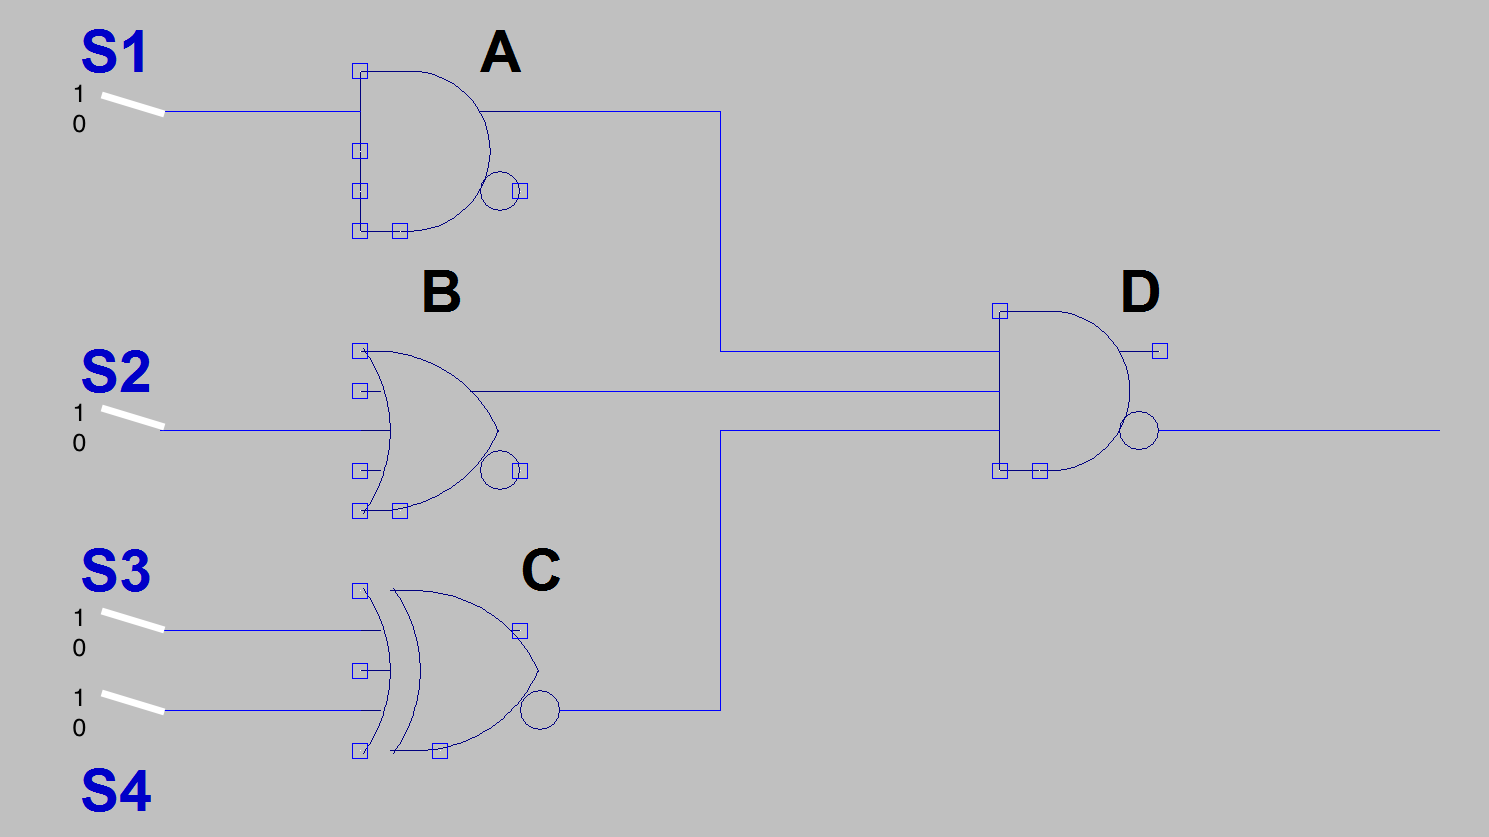
\includegraphics[width=0.8\linewidth]{circuit1.png}
  \caption{Circuit1}
  \label{fig:1}
\end{figure}

\newpage
\n\textbf{Circuit 2 definition file.}
\begin{lstlisting}[basicstyle=\small]
DEVICES CLOCK L 100, // clock output changes every 100 simulation cycles.
	SWITCH S1 1,
	SWITCH S2 0,
	SWITCH S3 0,
	DTYPE M,
	NOR A 2;
CONNECT S1 => M.SET,
	S2 => M.DATA,
	S3 => M.CLEAR,
	L  => M.CLK,
	M.Q => A.I1,
	M.QBAR => A.I2;
MONITOR A,
	QBAR;
/* A and QBAR are being monitored,
this is a multiline comment.*/
\end{lstlisting}
\begin{figure}[H]
  \centering
  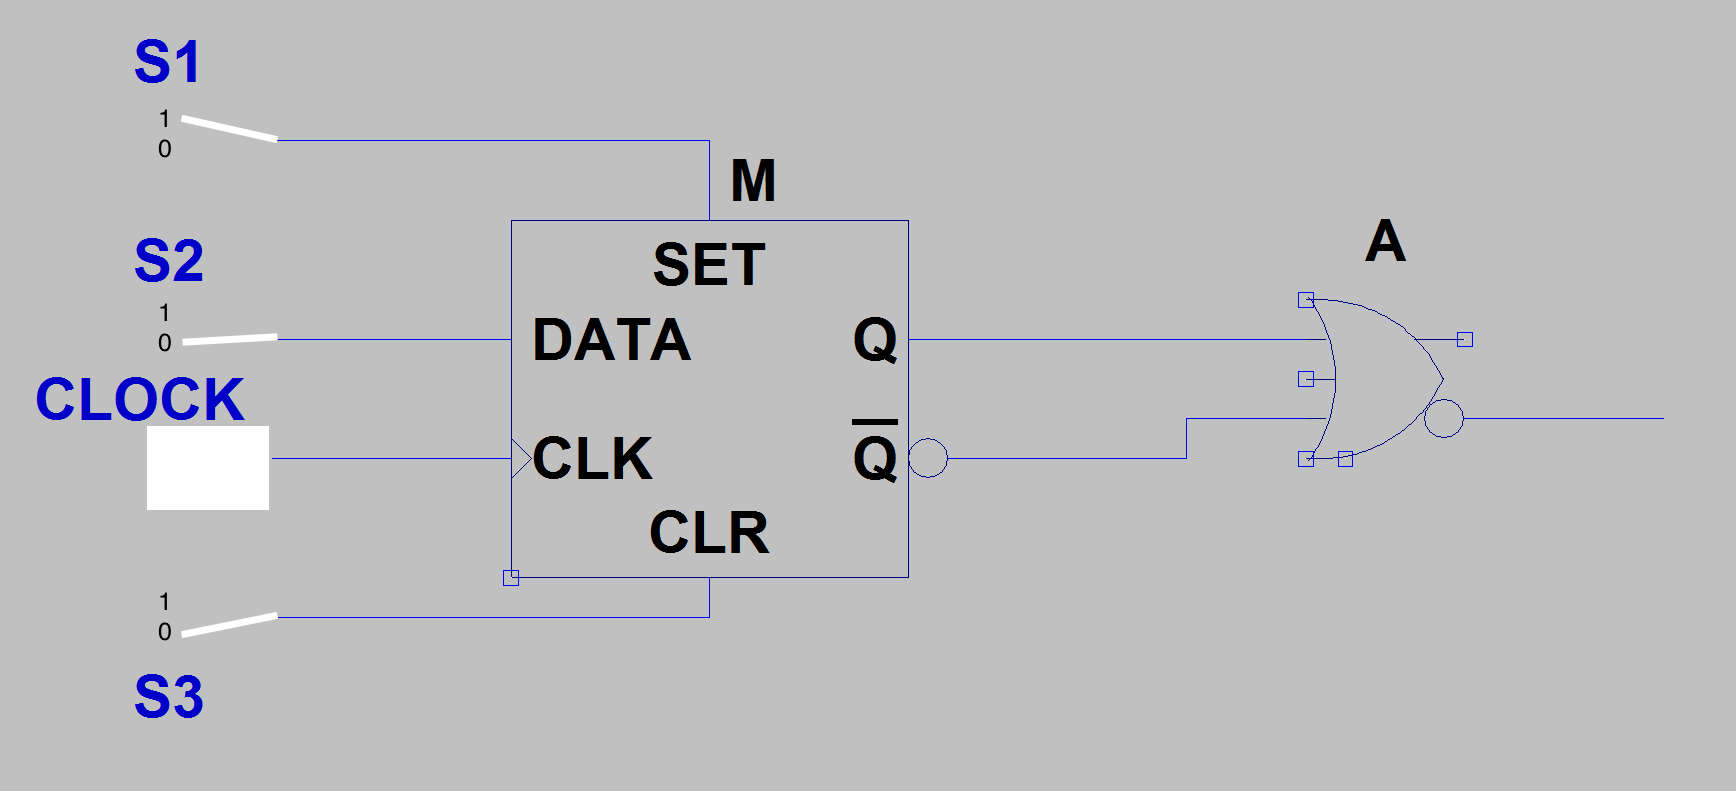
\includegraphics[width=0.8\linewidth]{circuit2.png}
  \caption{Circuit1}
  \label{fig:2}
\end{figure}

\end{document}